\documentclass[tikz,border=4pt]{standalone}
\usepackage{amsmath}
\begin{document}
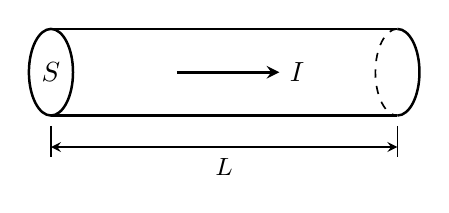
\begin{tikzpicture}[>=stealth, thick, scale=1.0]
  % Cylindrical conductor of cross-section S and length L carrying current I
  \draw[line width=0.9pt] (0, 0) ellipse (0.28 and 0.55);
  \draw[line width=0.9pt] (0, 0.55) -- (4.4, 0.55);
  \draw[line width=0.9pt] (0, -0.55) -- (4.4, -0.55);
  \draw[line width=0.9pt] (4.4, 0.55) arc (90:-90:0.28 and 0.55);
  \draw[dashed, line width=0.6pt] (4.4, 0.55) arc (90:270:0.28 and 0.55);

  \node at (0, 0) {$S$};
  \draw[->, line width=1.0pt] (1.6, 0) -- (2.9, 0) node[right] {$I$};

  % Length L dimension below
  \draw[line width=0.5pt] (0, -0.68) -- (0, -1.08);
  \draw[line width=0.5pt] (4.4, -0.68) -- (4.4, -1.08);
  \draw[<->, line width=0.6pt] (0, -0.95) -- (4.4, -0.95);
  \node[below, font=\small] at (2.2, -0.97) {$L$};
\end{tikzpicture}
\end{document}
